\begin{frame}[fragile]{Serial Loop Order \& Cache Misses}
    \begin{columns}[T]
        \begin{column}{0.495\textwidth}
            \centering{\textbf{\alert{Naive IJK Loop}}}
            \vspace{0.1cm}
            
            \begin{center}
                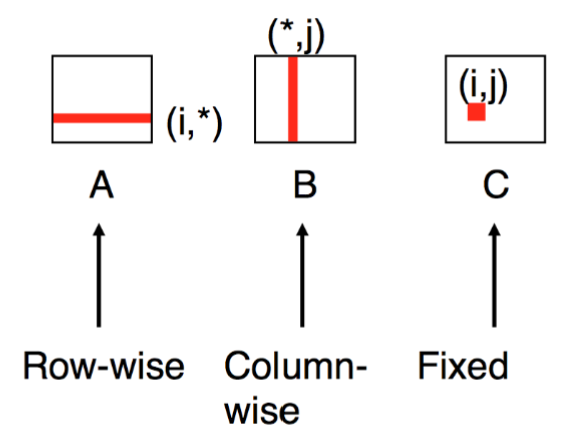
\includegraphics[width=0.7\textwidth]{Images/ijk_loop.png}
            \end{center}
            
            \begin{center}
                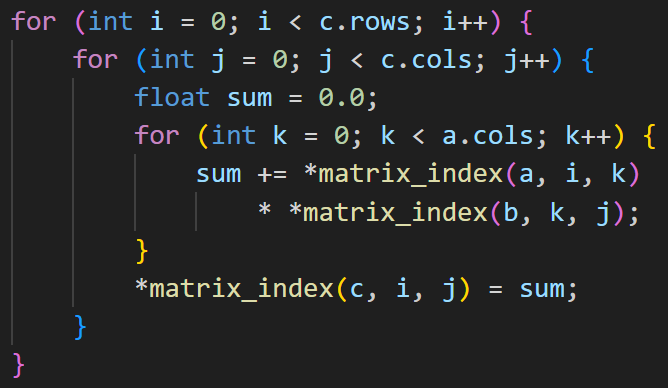
\includegraphics[width=0.85\textwidth]{Images/ijk_implementation.png}
            \end{center}
        \end{column}
        
        \hfill
        \vrule
        \hfill
        
        \begin{column}{0.495\textwidth}
            \centering{\textbf{\structure{Cache-Optimal IKJ Loop}}}
            \vspace{0.5cm}
            
            \begin{center}
                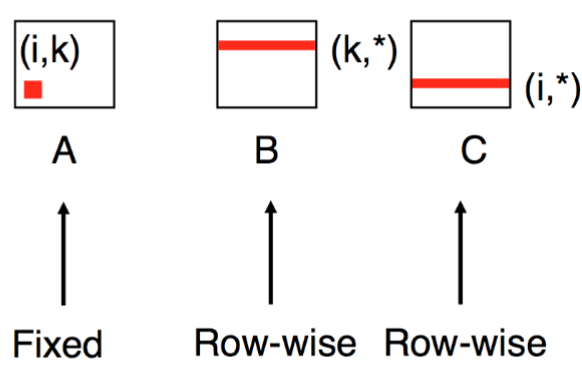
\includegraphics[width=0.7\textwidth]{Images/ikj_loop.png}
            \end{center}
            
            \begin{center}
                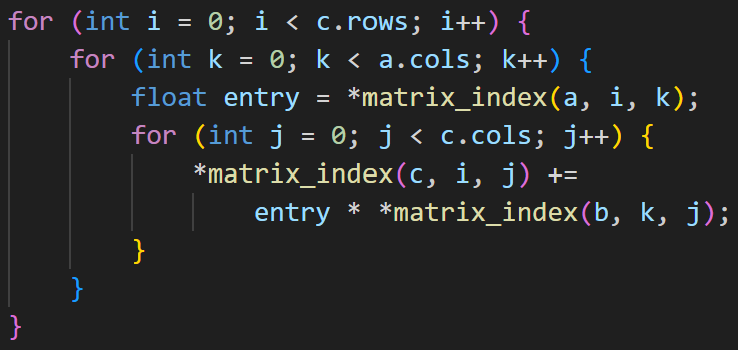
\includegraphics[width=0.95\textwidth]{Images/ikj_implementation.png}
            \end{center}
        \end{column}
    \end{columns}
\end{frame}


\begin{frame}[fragile]{Serial Optimal Cache-Oblivious Matrix Multiplication}
    \begin{columns}[T]
        \begin{column}{0.46\textwidth}
            
            \begin{center}
                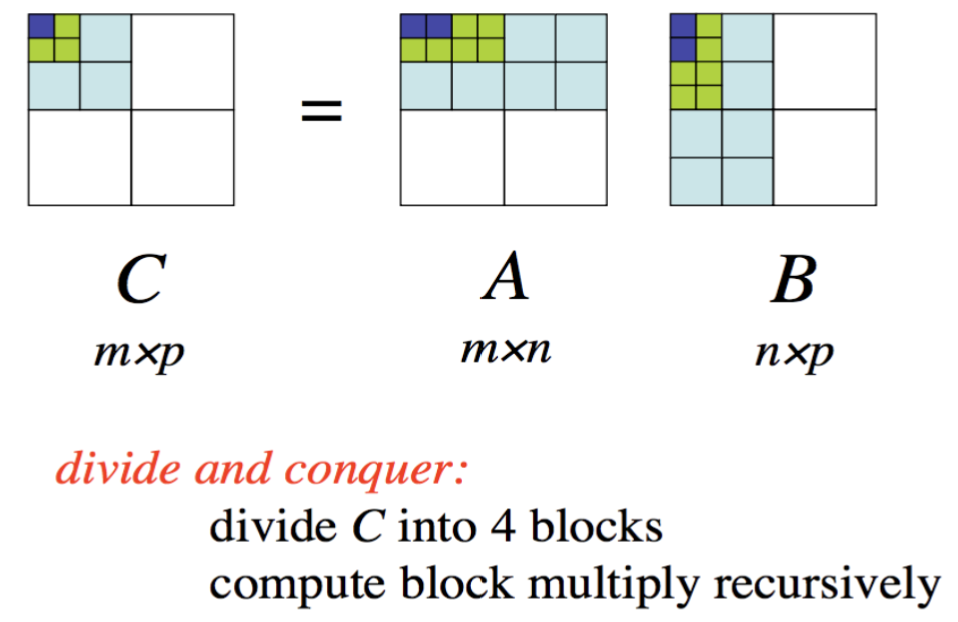
\includegraphics[width=0.95\textwidth]{Images/optimal_cache_oblivious.png}
            \end{center}
            
           
            
        \end{column}
        
        \hfill
        \vrule
        \hfill
        
        \begin{column}{0.50\textwidth}
             \begin{center}
                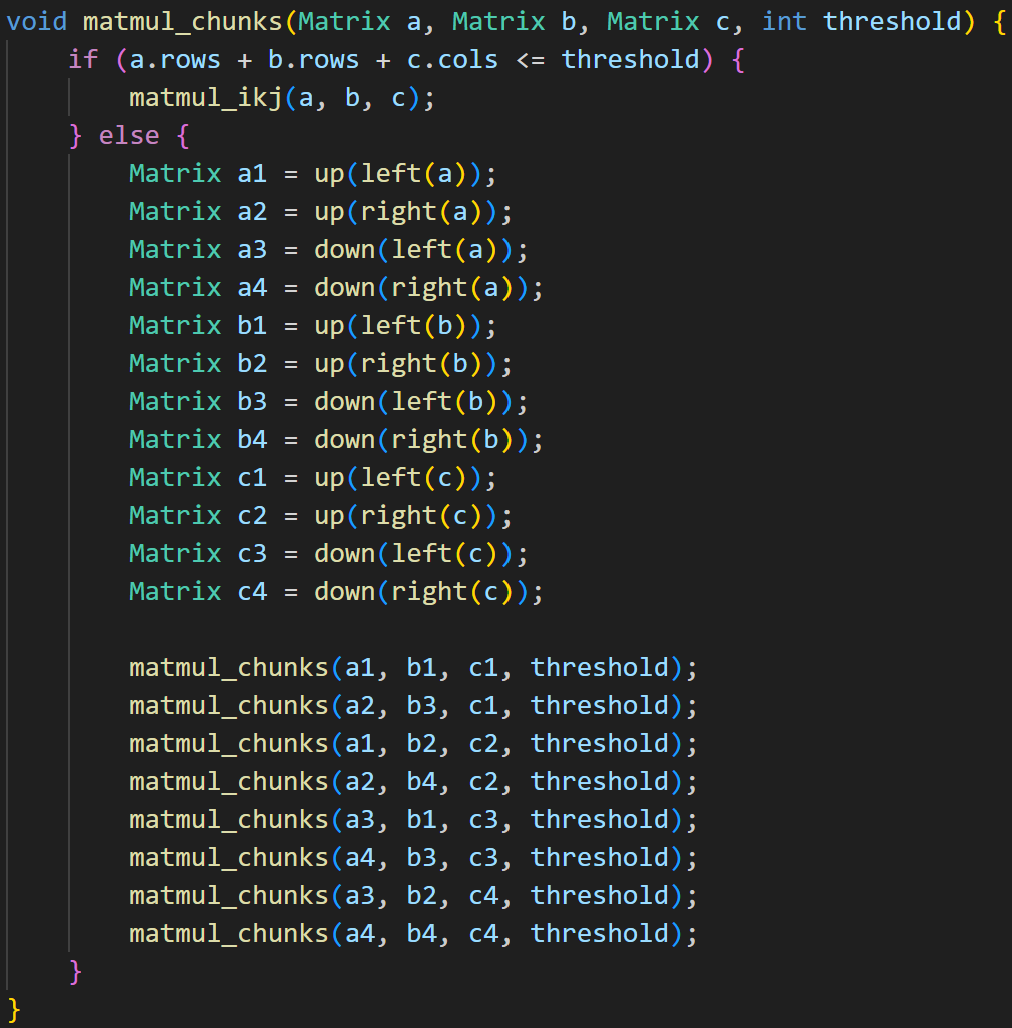
\includegraphics[width=0.75\textwidth]{Images/matmul_chunks.png}
            \end{center}
        \end{column}
    \end{columns}
\end{frame}

\begin{frame}{Serial Cache Miss Impact on Runtime}
    \centering Execution times are in seconds, averaged over 3 consecutive runs.
    
    \vspace{0.3cm}
    \centering
    \small
    \begin{tabular}{lrrrr}
        \toprule
        & \multicolumn{4}{c}{\textbf{Matrix Dimension ($N \times N$)}} \\
        \cmidrule(lr){2-5}
        \textbf{Algorithm Variant} & \textbf{1024} & \textbf{2048} & \textbf{4096} & \textbf{8192} \\
        \midrule
        IJK Loop          & 6.11 s        & 61.28 s       & ---           & ---      \\
        Transposed        & 0.65 s        & 5.48 s        & 47.31 s       & ---      \\
        IKJ Loop          & 0.14 s        & 2.08 s        & 15.73 s       & 140.13 s \\
        Chunks            & 0.26 s        & 2.13 s        & 17.71 s       & 144.02 s \\
        \bottomrule
    \end{tabular}
    
\end{frame}